\listfiles
\documentclass{article}
\usepackage{lipsum}
\usepackage[margin= 1 in, includefoot]{geometry}
\usepackage{graphicx}
\usepackage{hyperref}
\usepackage{xspace}

%Header and Footer stuff 
\usepackage{fancyhdr}
\pagestyle{fancy}
\renewcommand{\headrulewidth}{0 pt}
\renewcommand{\footrulewidth}{0.5 pt}

\begin{document}
\begin{titlepage}
\begin{center}

\huge{\bfseries Short-Term Load Forecasting using}\\
\huge{\bfseries ML \& Statistical Methods}\\
%[0.5cm]
\vspace{0.2in}


\includegraphics[scale=1]{IIT_Delhi.png}


\vspace{0.2in}
\large{\bfseries Project Supervisor:Dr V.V.K. Srinivas Kumar}\\
[0.1 in]

\large {\bfseries Department of Mathematics}\\
\large{\bfseries Indian Institute of Technology Delhi}\\
[1 cm]

\large{\bfseries Internal Supervisor: Dr Kusum Kumari Bharti }\\
[0.1 in]
\large {\bfseries Department of Computer Science}\\
[1cm]

\large{\bfseries By: Shivkumar Shinde}\\
\large{\bfseries Roll Number: 2016245}\\
[0.1 in]
\large{\bfseries Department of Mechanical Engineering}\\
[1cm]

\large{\bfseries Indian Institute of Information Technology, Design  and Manufacturing, Jabalpur}\\
[2cm]
\large{\bfseries December 2020}

\end{center}
\end{titlepage}


\section*{ABSTRACT}
\addcontentsline{toc}{section}{\numberline{}Abstract}
\large\mdseries{Short-term load forecasting is the basis for the safe operation of power systems. The accuracy of load forecasting will impact on the management of load distribution of the entire power grid. For a power grid, the capability to forecast load demand distribution in advance provides valuable decision supports. This review article studies real-time forecasting system of electricity load demand based on traditional(statistical methods) and non-traditional(machine learning approaches). Traditional researches usually examine models by setting up an evaluation metric and testing the overall forecasting performance of each model, finally the best model is selected. However the best model might be changing form time to time,since the load demand patterns are sensitive to the dynamic factors such as date, time, weather, events and so on. Here,we first study some statistical methods and their applications to load forecasting as a foundation for further research. Then we discuss machine learning approaches to forecast load demand, in which the pros and cons of each proposed model are analyzed. Beyond single models, we build a ensemble model that makes several single models work together in order to improve the forecasting accuracy. Finally, all the forecasting approaches are evaluated in a case study over energy market authority of Singapore. Experiments are conducted to simulate the operation of real-time forecasting system. From results we conclude that machine learning approaches are better for forecasting load.
}

\newpage
\begin{center}
\section*{ACKNOWLEDGEMENT}
\addcontentsline{toc}{section}{\numberline{}Acknowledgement}
\end{center}
\large\mdseries{I would like to express my special thanks of gratitude towards Dr V.V.K.Srinivas Kumar for their able guidance and support in completing my project. I feeling oblige in taking opportunity to sincerely thanks to Prof. Aparijita Ojha and Prof. Kondekar Pravin N for providing me with all the facility that was required and helping me to make improvement on this project. At last but not the least I am thankful to all faculty members, friends and specially my family who have been always helping and encouraging me throught the year. 
}\\
[2 cm]
\textbf{
\begin{flushright}
\large\mdseries{Shivkumar Shinde}\\
\large\mdseries{2016245}\\
\large\mdseries{Department of Mechanical Engineering}\\
\large\mdseries{Indian Institue of Information Technology, Design and Manufacturing, Jabalpur}\\
\end{flushright}
}

\newpage
\begin{center}
\section*{Author's Declaration}
\end{center}
\large\mdseries{
I, Shivkumar Shinde(2016245) the undersigned, hereby declare that this submission is entirely my own work, in my own words, and that all sources used in researching it are fully acknowledged and all quotations properly identified.  It has not been submitted, in whole or in part, by me or another person, for the purpose of obtaining any other credit / grade.  I understand the ethical implications of my research, and this work meets the requirements of the faculty of Computer Science and Mechanical Engineering Department.
}

\textbf{ 
\begin{flushright}
\large\mdseries{Student Name: Shivkumar Shinde}\\
\large\mdseries{Roll Number: 2016245}\\
\end{flushright}
\large\mdseries{Signed: 
}
}

\newpage
\tableofcontents
\addcontentsline{toc}{section}{\numberline{}Table of Contents }
\newpage
\listoffigures
\addcontentsline{toc}{section}{\numberline{}List of Figures}

\newpage
\section{Introduction}  
\large\mdseries{Electricity is an essential part of modern life and important to a nation's economy. It is used for different purposes like residential use, industrial use, transportation and commercial buildings. In order to provide customers safe and stable eletricity, an electric power company need effective schedules but in process it faces too many problems.

                Smart grids which are known to have features including reliability, flexibility, sustainability, and efficiency, have emerged as a solution for numerous current problems, including energy shortage and environmental pollution. To get more effective schedules, we need short-term load forecasting(STLF). Short-term load forecasting is an integral part of the energy planning sector. Designing a time ahead power market requires demand scheduling for various energy divisons, namely generation, transmission and distribution. It helps power system operators with various decision making in the power system, including supply planning, generation reserve, system security, dispatching scheduling, demand-side management, financial planning, and so forth. Accurate forecasts lead to substantial savings in operating and maintenance costs, increased reliability of power supply and delivery system. Otherwise inaccurate demand forecasting will cost the utility a tremendous financial burden.\cite{fallah2019computational}.
                
                Load forecasting is classified in three categories accroding to planning horizons duration as: 1 day/week ahead for short-term, 1 day/week to 1 year ahead for medium-term, and 1 year ahead for long-term. Short-term forecasts are used to schedule the generation and transmission of electricity. Medium-term forecasts are used to schedule the fuel purposes. Long-term forecasts are used to develop the power supply and delivery system.
                
                STLF is not an easy task because energy consumption pattern are complex, and uncertain external factors can cause a shift in the demand curve. Demand pattern affected by factors including architectural structure, special events, resident schedules, environment and lighting. Social and environmental factors are the big resources for the randomness found on the load pattern. Complexity in load pattern have been leading to develop complicated methods of forecasting. This lieturature is containing electric load forecasting methods with attempts to find best estimation of load forecasting. The major methods include time series such as Naive approach, Moving average, Simple Exonential Smoothing, Holt's linear trend model, Holt's winter model, ARIMA, and neural networks. Sequential models like Long Short Term Memory (LSTM) come into picture for better estimation of electric load.
                
                Time series methods and ARIMA model have achieved a considerable success for electric load forecasting. In general, ARIMA model is used when time series is stationary and data is not missing. To date, numerous artificial neural network(ANN)-based STLF models have been constructed to predict exact electric loads and have exhibited favorable performance. To further improve their performance, it is critical to effectively tune their hyperparameters to specify the structure of the network itself or to determine how to train neural network(NN).
                
                Though there are many forecasting methods, no single one can be generalised to perform enough for all cases, especially when many factors are considered. In other words, an ideal method for one case may perform poorly for another. So research must be directed for specially assigned methods.
                
}  
\newpage
\large\mdseries{In this article our aim is to demonstrate pragmatic forecasting methodology for analyzing the load pattern and predicting the future demand for short-term. This methodology can integrate many forecasting models.

                The rest of the article is organized as follows. In section ``Data Collection'', we describe dataset used for proposed methodoligies. In section ``Forecasting Methods'', we demonstrated the 30 min interval electric load forecasting methods based on time series methods and neural networks. In section ``Results \& Conclusions'' we described the results obtained by the forecasting model implemented on the dataset and conclude the results. By observing results we proposed future study directions.   
 }
 
 
\newpage
\section{Data Collection}
\large\mdseries{ We are using load data collected from Energy Market Authority, Singapore. Load data is available at a time step of 30 minutes, totally 48 values for a single day. We took data for time period of a week from (2-11-2020 to 8-11-2020) and then again collected data from (7-12-2020 to 20-12-2020). Here we presented general trend of the data in folloeing plot for data from (7-12-2020 to 20-12-2020).
\\
[1 cm]

\begin{figure}[h]
\centering{
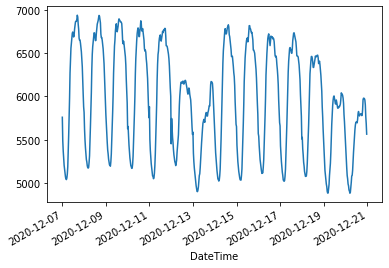
\includegraphics[width = 1\textwidth]{December2020.png}}
\caption{\label{fig:my-label} Time Series Data Plot (Half Hourly Data)}
\end{figure}

\newpage
\section{Forecasting Methods \& Methodology}
\large\mdseries{ In this review article we discussed forecasting methods, from moving average, Holt's methods to artificial neural networks and recurrent neural networks. We discussed all these methods thoroughly.
\subsection{Naive Approach:}
\large\mdseries{ In this method, we assume the next expected point is equal to last observed point,so here we can expect a straight line as prediction result for the given duration.
\subsection{Moving Average:}
\large\mdseries{ In this forecasting technique, we take average of the last few time periods. Here we took  average of last few data points as a prediction result for the given duration. We used python dataframes rolling mean of window size of 3 data points to get average and use it to forecast the future values. }
\subsection{Simple Exponential Smoothing:}
\large\mdseries{ In this model, we assign weights from the recent obeservations to older observations with the help of alpha (Smoothing constant or learning rate) and forecasts the future demand with the help of following equation. The underlying idea behind this model is that, at each period model will learn a bit from the most recent demand observation and remember a bit of last forecast it did.
$$ f_{t} = \alpha Y_{t} + (1-\alpha) f_{t-1}  $$
where  $f_{t}$ is forecast at time t, $\alpha$ is a smoothing constant which is in the range 0 to 1, $Y_{t}$ is recent observation (demand) and $f_{t-1}$ is previous forecast.
Here we used python's statsmodels library to fit and predict the values.
}
\subsection{Holt's Linear Trend Model:}
\large\mdseries{ In this model, we forecast the future values by capturing the trend, and this is dobne by adding a second single exponential smoothing model to the simple exponential smoothing model. Equations of the model as follows:
$$ u_{t} = \alpha Y_{t} + (1-\alpha) (u_{t-1}+v_{t-1})  $$
$$ v_{t} = \beta(u_{t}-u_{t-1}) + (1-\beta)v_{t-1} $$
$$ y_{t+h|t} = u_{t} + hv_{t} $$
where $\beta$ is smoothing constat same as alpha and $0\leq\beta<1$. Here we used python's statsmodels library to fit and predict the values.}
\subsection{Holt's Winter Model:}
\large\mdseries{ In this method of forecasting, we forecast the future values by capturing the trend and seasonality from the time series. Equations of the model are as follows:
$$ l_{t} = \alpha(y_{t} - s_{t-m}) + (1-\alpha)(l_{t-1}+b_{t-1})  $$
$$ b_{t} = \beta(l_{t} - l_{t-1}) + (1-\beta) (b_{t-1}) $$
$$ s_{t} = \gamma(y_{t} - l_{t-1} - b_{t-1}) + (1-\gamma)s_{t-m} $$ 
$$ y_{t+h|t} = l_{t} + hb_{t}+s_{t+h-m(k+1)} $$

where k is integral part of $ \frac{h-1}{m} $. The above three equations represent $l_{t}$  for the level, $ b_{t} $ for trend and $s_{t}$ for seasonality. $ \alpha, \beta, \gamma $ are smoothing constants, m represents the frequency of seasonality for instance quarterly data m = 4, monthly data m= 12 and weekly data m = 7 and h represents the time interval. 
     }

\subsection{Auto-Regressive Integrated Moving Average (ARIMA)}
\large\mdseries{ARIMA models are widely used for time series forecasting and it mainly describes the autocorrelation between the data. The components of ARIMA model are explained as:

               \textbf{Auto-Regression AR :} In this model we forecast the variable of interest using past values of the variable i.e. regression against itself or it's lagged values. The auto-regressive model of order p can be written as:
       $$ y_{t} = c + \phi_{1}y_{t-1} + \phi_{2}y_{t-2} + ... + \phi_{p}y_{t-p} + \varepsilon_{t} $$
               
               \textbf{Integrated I :} This is technique of differencing observations i.e. time series data points to make time series stationary. Data points are replaced with difference between consecutive values. Order of difference is denoted by d.\\
               
               
               \textbf{Moving Average :} In this method we forecast the future values by taking linear function of past errors into account. Moving average model of order q is defined as follows:
       $$ y_{t} = c + \varepsilon_{t} + \theta_{1}\varepsilon_{t-1} + \theta_{2}\varepsilon_{t-2} +...+ \theta_{q}\varepsilon_{t-q} $$
                 
                \textbf{Model Architecture :} Here we have load data in terval of 30 minutes or half hourly period. We implemnted individual AR and MA model to forecast the future values and integrated these models to implement (for training and prediction) ARIMA model using python's statsmodels library. As we are getting high root mean square error, a metric used to evaluate model's performance, we used python's autoarima library to check best fit model for our data, we got the model and used it for training and prediction with the help of python's statsmodels library. 
 }     

\subsection{ANN (Feed Forward Neural Network FFNN) :}
\large\mdseries{ FFNN is an artificial neural network (ANN), which is mutli layer perceptron. It consists of an input layer, one or more hidden layers and an output layer. In this network information flows only in one direction from input layer(nodes) through hidden layers (hidden nodes) to output layer(output node). Each layer comprises of number of nodes. Each node gets values from previous nodes and applying specified function produces its output and passes it to nodes on the next layer. At last nodes at output layer produces the output. We defined a loss function accroding to our output requirement and to minimize the loss we use adam learning algorithm. With the help of learning algorithm we update the parameters and calculate loss, this process is repeated and we get desired output.  \cite{moon2019comparative}.

\begin{figure}[h]

\centering
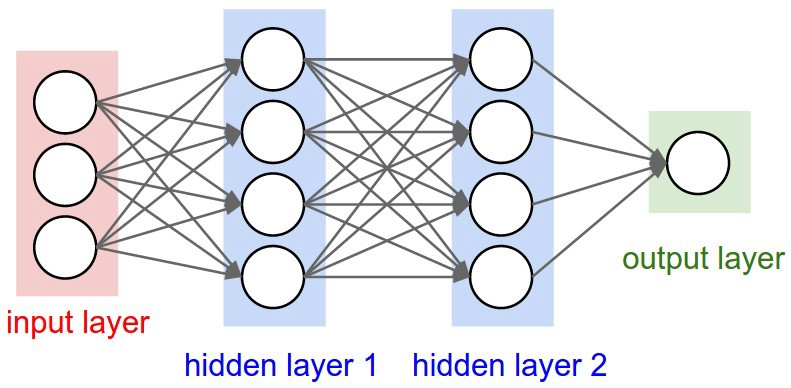
\includegraphics[width = 0.5\textwidth]{FFNN(10,64,64,1).jpg}
\caption{\label{fig:my-label} FFNN (10,64,64,1)}

\end{figure}

                 \textbf{Model Architecture :} In above figure no.2 we have explained our model configuration, it consists of input size of a vector containing 10 data values and feed to the model as sequential data and it has 2 hidden layers consisting 64 nodes each which gives 64 output values to the next layer and last one output layer containg one node giving one desired output. The two dense layer (hidden layers) are having rectified linear unit (relu) as a activation function, followed by another dense layer containg only one node without any activation function. Metric used for loss is mean squared error optimized with adam optimizer. The model was trained for 25 epochs using python's keras library. 
     }
     
\subsection{Recurrent Neural Networks (RNN):}
\large\mdseries{  Some tasks need to be able to process the information better, that is, previous input is related to subsequent input. For example when we need to understand the whole sentence, it is not only important to understand each word,but also we need to deal with the whole sequence of these words. At this time, we need another significant neural network in the field of deep learning: Recurrent Neural Network.
Basically RNN is generalization of feed forward neural network, which models the tasks which involve sequences by adding recurrent neural network. In such networks we can handle the dependence between inputs, variable number of inputs and at each time step function calculating the output is same. The output calculated at current time step depends not only on the current input but also on the previous input, in this way function calculating output at certain time step contains all the information from the starting time step. We can call it as rnn deals the information with help of internal memory, which is finite.
\begin{figure}[h]

\centering
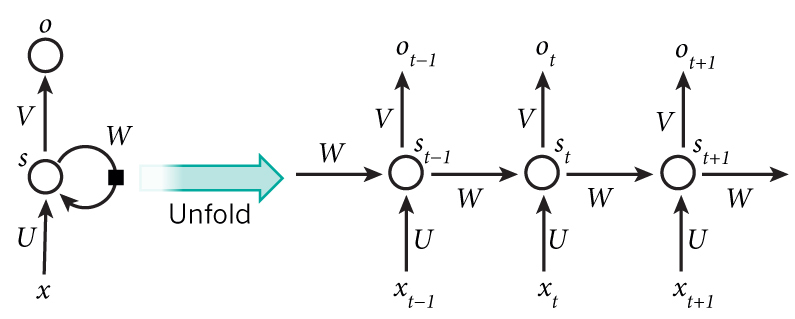
\includegraphics[width = 0.5\textwidth]{rnn.jpg}
\caption{\label{fig:my-label} Recurrent Neural Network}

\end{figure}
 

The above figure is a simple rnn, which consists of an input layer, a hidden layer and an output layer. It handles sequential data and its output is affected by previous input values. The learning algorithm used to train rnn is backpropagation through time (BPTT), when we used the BPTT learning algorithm, came across the problem of exploding and vanishing gradient and it lead to the introduction of long short term memory(LSTM).
}
\subsection{Long Short Term Memory (LSTM):}


\large\mdseries{ Long Short Term Memory Algorithm(LSTM), which successfully solves the defects of original cyclic neural network, has become the most popular RNN and has been successfully applied for speech recognition, picture description and natural language processing.\cite{yang2019electric}.
                 
                 With the help of LSTM, the problem of exploding and vanishing gradients which occurs in ordinary rnns can be solved quite efficiently. The problem of exploding gradient is easier to handle, we can normalize the gradient as we are interested only in the direction of the gradient. The vanishing gradient problem is difficult to handle and LSTM networks can overcome this with the help of processing information in a way such that selective read the information, selective write information and selective forget information at each time step. This is more formally done by the concept of gates; input gate, forget gate and output gate.
                 
                 The problem of vanishing gradient, which occurs in ordinary rnns can be overcome with the help of these gates. Actually what happens, at further time steps infomation contained, the contribution of initial time steps becomes very small and during learning the parameters, it get vanished and error occured due to that time step can not be resolved. So in order to resolve this problem we use LSTM cell. 
                 
                 LSTM in itself saying that it remebers its input over a long period of time with the help of memory which is called gated cell. This gated cell decides which information has to be read, forget and write with the help of assigning importance to the information which can be done by introducing weights, which are also learned by modelling it into parametric form and then learn these parametres with the help of same learning algorithm.
                 
                 LSTM consists of three gates input gate, forget gate and output gate. Input gate decides whether or not to allow new input, forget get decides which information is not important and delete it and outout get decides that whether or not input impacts the output at current time step.  
}\\

\begin{figure}[h]

\centering
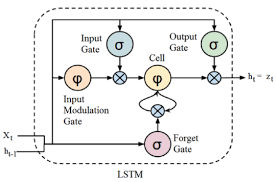
\includegraphics[width = 0.5\textwidth]{LSTM_Cell.png}
\caption{\label{fig:my-label} Long Short Term Memory}

\end{figure}

                \textbf{Model Architecture :} The model consists of one LSTM cell with hyperbolic tangent (tanh) function as activation function followed by 2 dense layers without any activation function. Metric used for evaluating performance of model is root mean squared error (RMSE). The model was trained for 50 epochs. The code was written in Python using Keras library.

\subsection{Methodology :}
\large\mdseries{ We prepared dataset according to our requirement which is collected form Energy Market Authority, Singapore. For non-traditional methods we split dataset into train, validation and test datasets. We trained our forecasting model on train dataset and check its performance on the validation dataset with the help of metric used is root mean squared error. If performance is well then we use that model to forecast day ahead values for test dataset. 

                 For artificial neural networks method we split dataset into train and test datasets, scale the values to range(0,1) in order to optimize the performance. Here train our model on training datset and predict day ahead values on test dataset and evaluate model's performance with the help of metric root mean squared error(RMSE).
                 
}

\section{Results \& Conclusions :}
\large\mdseries{  In this section results of the above mentioned methodologies are discussed. We implememnted Naive approach, Moving average, Simple Exponential Smoothing, Holt's Linear Trend Model, Holt's Winter Model and ARIMA Model. The dataset used collected from Energy Market Authority, Singapore from 07-12-2020 to 20-12-2020, each day containing half-hourly (an interval of 30 minutes) data. We make predictions on validation dataset containing time interval (16-12-2020 19:30 to 19-12-2020 14:00). 

                  We make prediction using python's statsmodels library, and calculated root mean squared error (RMSE) value, metric used for evalution of model's performance. we got high RMSE value for above methods except for Holt's winter model, which is a bit large too. We make prediction using ARIMA model and  it's individual components Auto-Regression(AR) and Moving Average(MA) models used for prediction on validation dataset too, but we got large RMSE values. We alos tried AUTOARIMA model which tells us the right model configuration for best fit of values on training and gives accurate predictions, but we got high RMSE in this case too.
\\                  
                  
\begin{figure}[h]

\centering
\includegraphics[width = 0.5\textwidth]{Holt's Winter.png}
\caption{\label{fig:my-label} Holt's Winter Forecast}

\end{figure}
                 
                 
                 
The above figure shows Holt's Winter model's forecast for the time period (16-12-2020 19:30 to 19-12-2020 14:00 ). This is half hourly prediction, y-axis contain forecasted electricity load denoted by red line in  MW unit and x-axis contain index of validation dataset on which prediction is done. RMSE value for this model is 209.2447.

After using these time series methods we used non-traditional artificial neural network techniques (ANN) for the forecasting of day ahead values on test dataset. First we applied these ANN and RNN models to short length dataset of time intervel (one week 02-11-2020 to 07-11-2020) but we got poor results and then we incresed the length of dataset for 2 weeks of time interval (07-12-2020 to 20-12-2020). we made predictions on test dataset of time interval (16-12-2020 11:00 to 20-12-2020 00:00). RMSE for Feed Forward Neural Network (FFNN) is 52.54 and RMSE for Long Short Term Memory (LSTM ) is 65.61.


\begin{figure}[h]

\centering
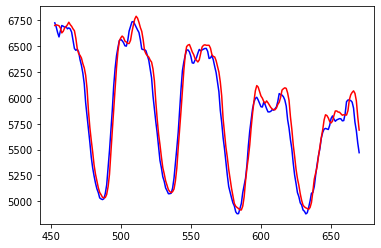
\includegraphics[width = 0.5\textwidth]{FFNN.png}
\caption{\label{fig:my-label} Feed Forward Neural Network Forecast}

\end{figure}

The above figure shows FFNN's forecast(denoted by red line) for the time interval (16-12-2020 11:00 to 20-12-2020 00:00).
\\


\begin{figure}[h]

\centering
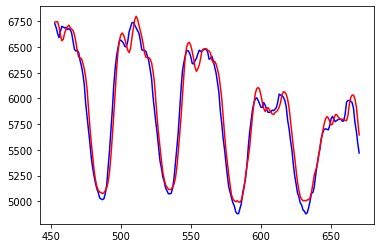
\includegraphics[width = 0.5\textwidth]{LSTM_result.png}
\caption{\label{fig:my-label} Long Short Term Memory Forecast}

\end{figure}

The above figure shows Long Short Term Memory's forecast(denoted by red line) for the time interval (16-12-2020 11:00 to 20-12-2020 00:00).

The below table shows the error metric for the time interval (16-12-2020 11:00 to 20-12-2020 00:00).

\begin{table}[ht]

  \centering
  \begin{tabular}{|c|c|c|}
  \hline
  Sr.no. & Methods & RMSE \\
  \hline
  \hline
  1 & Holt's Winter & 209.2447 \\
  \hline
  2 & FFNN & 52.54 \\
  \hline
  3 & LSTM & 65.61 \\
  \hline
  \end{tabular}
  \caption{Metric Table}
  \label{Metric Table}
\end{table}


               \textbf{Conclusion}{ In this project we implemented Naive approach, Moving Average, Simple Exponential Smoothing, Holt's Linear Trend Model, Holt's Winter Model, ARIMA Model, FFNN Model, and LSTM Model. Performance of models is different and  Holt's Winter Model, FFNN Model and LSTM model are among them best performing models. Performance of these models can be further improved by increasing datapoints, incorporating weather parameters. Results of these models are in fine range and there is no very sharp fluctuations.}
               
}
}

\bibliographystyle{elsarticle-num}
\bibliography{mybib}@MastersThesis{yang2019electric,
author = {Yang, Tianshu},
title = {Electric Load Forecasting Using Long Short-term Memory Algorithm},
year = {2019}
}


\end{document}